For over a century, researchers have tried to understand the impact of mutations on an individual's selective value. However, this understanding remained limited, in particular because experimental techniques did not allow the appearance of new mutations to be observed directly, or their effects to be measured precisely. 

In a 2018 article, Robert and al. \cite{robert2018mutation} propose to overcome this difficulty by describing a new experimental method that makes it possible to see the appearance of new mutations in real time. In the same article, they explain second experimental method for estimating the selective value of a cell line over time.
These new techniques provide new data for understanding more precisely the impact of mutations on an individual's selective value. \\

In this section, we present the experimental techniques presented in \cite{robert2018mutation} as well as the available data.

\section{Detect mutations : \emph{Mutation Visualisation experiment}}

    \subsection{The Mismatch Repair}
    
Deoxyribonucleic acid (DNA) is a double-helix molecule that carries genetic information. It is an extremely precise piece of machinery, which means that the slightest disturbance to one of its strands is likely to alter the behaviour, and therefore the ability, of the cell to survive. \\

To avoid such events, living cells have developed complex repair systems capable of recognising and correcting these disturbances. When these systems correctly eliminate the disturbance, there are no consequences for the cell. On the other hand, when the repair system fails to eliminate the disturbance, a mutation occurs. \\

\subsubsection{DNA replication} During DNA replication, the two strands are separated by an enzyme: \emph{DNA Polymerase}. These strands (matrices) enable two new identical DNA helices to be reconstructed by base complementarity. The new strand is determined by the old strand: an A base on the mother strand will ensure a T base on the new strand, etc. (Figure \ref{fig:replication_adn}).

\begin{figure}
    \centering
    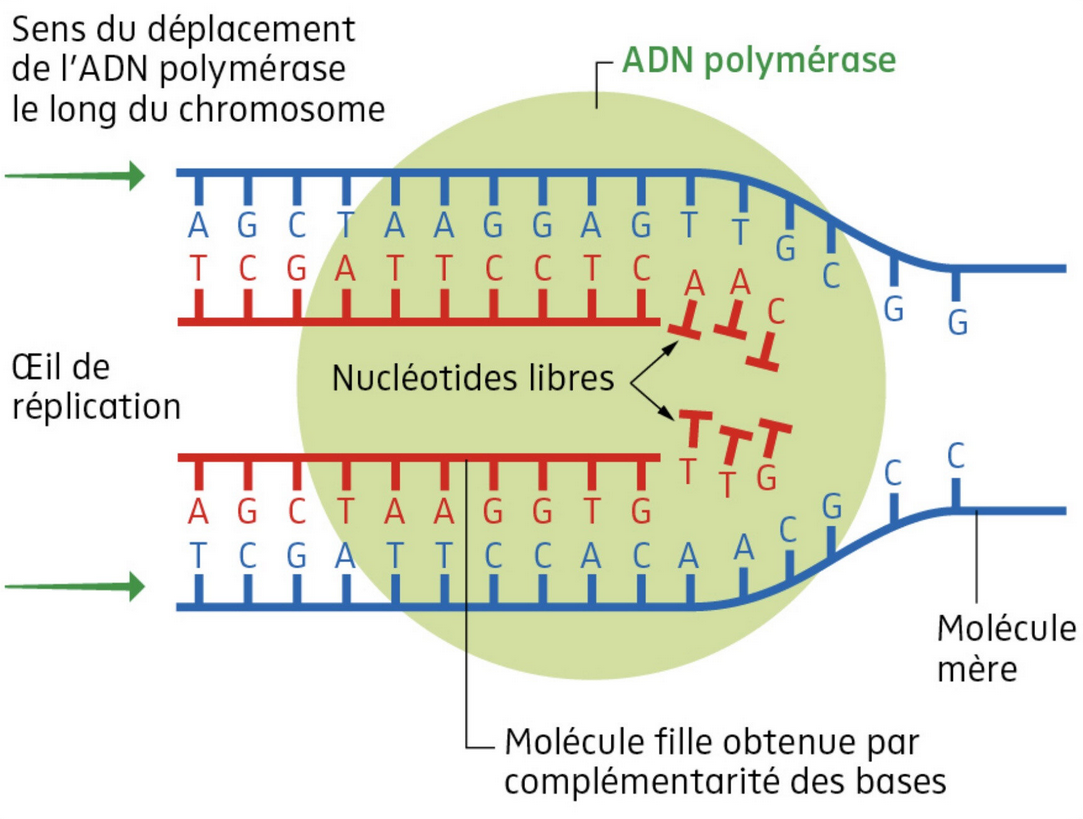
\includegraphics[width=0.5\textwidth]{pictures/replication_ADN.png}
    \caption{Simplified representation of a replication fork. Note that the new strands are complementary to the old strands. \\
     \ndr{Faire une image en anglais}}
    \label{fig:replication_adn}
\end{figure}

Sometimes a replication error occurs. In this case, one of the bases of the new strand is not complementary to its associated base. This is known as a mismatch. (Figure \ref{fig:mesappariement}).

\begin{figure}
    \centering
    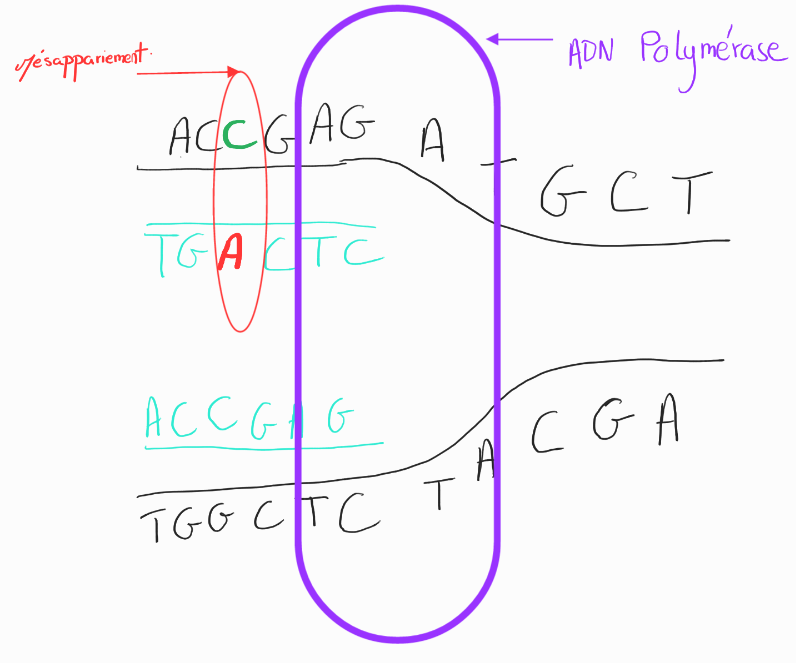
\includegraphics[width=0.5\textwidth]{pictures/mesappariement_adn.png}
    \caption{Artistic representation of a mismatch. A base G has been transformed into a base A.}
    \label{fig:mesappariement}
\end{figure}

\subsubsection{Mismatch detection and repair} 
The DNA Mismatch repair (MMR) is monitoring mechanism used during replication \cite{iyer2006dna}. It detects and repairs mismatches committed by the DNA polymerase during the replication process. The MMR system best known today is that of Escherichia coli, known as the MutHLS system, comprising the MutH, MutL and MutS proteins. \\

The repair system. The MutS protein recognises the mismatch and the MutL protein confirms the mismatch, then both bind to the DNA. The accumulation of MutS and MutL proteins activates the MutH protein, which cuts the neosynthesised strand. Resynthesis is then possible. (Figure \ref{fig:syst_mutHLS})

\begin{figure}
    \centering
    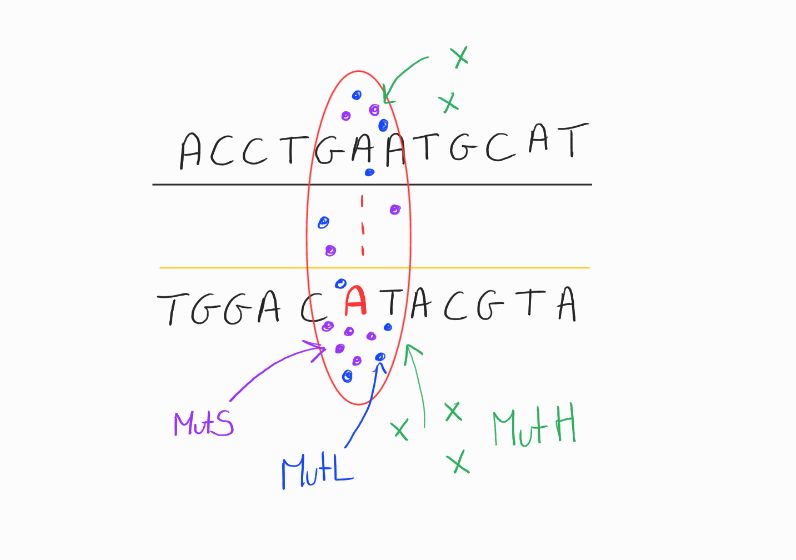
\includegraphics[width=0.8\textwidth]{pictures/syst_MutHLS.png}
    \caption{Schematic representation of the action of the mutHLS system.}
    \label{fig:syst_mutHLS}
\end{figure}


\subsubsection{The emergence of a mutation}

A mutation occurs when the mismatch repair system fails to repair a mismatch. In this case, the newly formed DNA has two mismatched bases. During replication, the DNA polymerase will form two new strands, one of which will carry a mutation compared to the original genome.
    
    \subsection{Real-time mutation detection}
    
    In \cite{robert2018mutation}, the authors develop a new strategy to observe the appearance of new mutations in real time. \\
    To begin with, they add a fluorescent protein (YFP) to the MutL protein. As the MutL proteins accumulate around the mismatch sites, it is possible to see the appearance of a new mutation using imaging techniques. \\
    In addition, the MutH endonuclease is deactivated to ensure that the mismatch is not repaired (Figure \ref{fig:syst_mutHLSmodifie}).

\begin{figure}
    \centering
    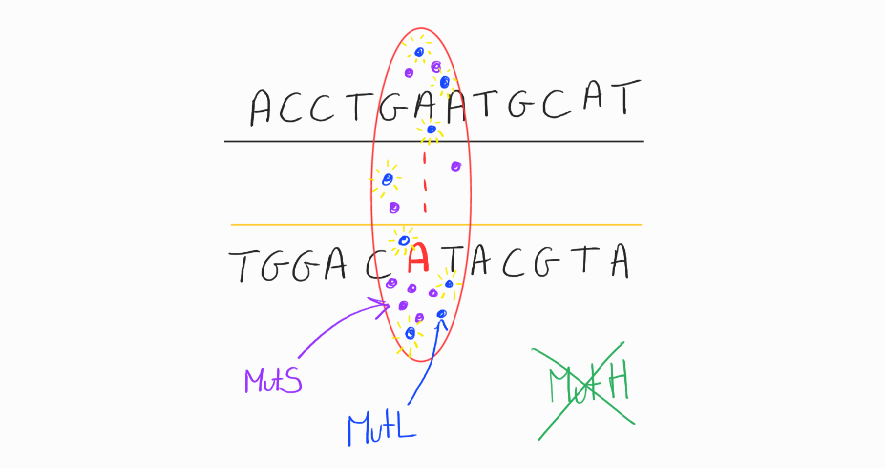
\includegraphics[width=0.8\textwidth]{pictures/syst_MutHLSmodifie.png}
    \caption{Schematic representation of the MV experiment}
    \label{fig:syst_mutHLSmodifie}
\end{figure}

\subsection{Discussion}

Using the results obtained in \cite{robert2018mutation}, the authors argue that the emergence of new mutations follows a Poisson process. 

\section{Measuring fitness: \emph{microfluidic Mutation Accumulation ($\mu$MA) experiment}} 

Mutation accumulation (MA) is the classic method for directly studying the effects of mutation \cite{mukai1964genetic,halligan2009spontaneous}. Several colonies of cells are derived from a single common ancestor. When the colonies have reached a sufficient size, a cell is randomly drawn from each colony to form a new one. \ndr{Mettre une figure}.
Several studies combine MA experiments with genome sequencing to estimate the rate and effects of mutations \cite{lynch2016genetic,tenaillon2016tempo} and MA experiment has been used to study mutations for several species \cite{katju2019old,ossowski2010rate,rutter2012fitness, baer2005comparative}. It is commonly assume that natural selection have no role in the evolution of colonies even if this method produces several selection biases that can skew the results \cite{mahilkar2022selection}. 

Microfluidic methods can be used to avoid these biases. The Microfluidic Mutation Accumulation ($\mu$MA) experiment is a technique developped in \cite{robert2018mutation,robert2019real} to study mutation rates, evolutionary dynamics and genetic stability in microorganisms. This experiment create a controlled environment where mutations can accumulate over successive generations without the selective pressures that typically eliminate deleterious mutations. By isolating and propagating single cells repeatedly, the µMA experiment allows to directly observe the effects of accumulated mutations on fitness, genome stability, and evolutionary trajectories, providing insights into how mutations contribute to genetic diversity and evolution. \\

In \cite{robert2018mutation}, the authors track the evolution of 1476 cell lines using microfluidic methods. For each new generation, only one daughter cell is kept, regardless of its fitness. \\
By filming the different cell lines over time, it is possible to measure changes in growth rates.

%\section{Description of the datasets}

